\documentclass{article}
\usepackage{fullpage}
%\usepackage{times}
\usepackage{url}
\usepackage{amsmath,amsthm,amssymb,color}
%\usepackage{multicol}
\usepackage{float}
\usepackage[section]{placeins}
\usepackage{graphicx}
\usepackage{hyperref}
\usepackage{courier}
\usepackage{listings}
\usepackage{color}
\definecolor{lightgray}{rgb}{.9,.9,.9}
%\usepackage[all]{hypcap}

\newcommand{\Squash}{\mathsf{Squash}}
\newcommand{\Clamp}{\mathsf{Clamp}}
\newcommand{\Range}{\mathsf{Range}}

\let\x\cdot
\lstset{
  language=Python,
  backgroundcolor=\color{lightgray},
  showstringspaces=false,
  tabsize=4,
  basicstyle=\ttfamily,
  keywordstyle=\bfseries\ttfamily,
  captionpos=b
}
\lstdefinelanguage{JavaScript}{
  keywords={if,else,var},
  keywordstyle=\bfseries\ttfamily,
  backgroundcolor=\color{lightgray},
  sensitive=false,
  comment=[l]{//},
  morecomment=[s]{/*}{*/}
}

\begin{document}

\title{\bf Range Analysis for the IonMonkey JavaScript engine}

\author{
Ryan Pearl\footnote{Equal contribution to this work}\\
\texttt{$<$rpearl@andrew.cmu.edu$>$}\\
\and
Michael Sullivan\footnotemark[\value{footnote}]\\
\texttt{$<$mjsulliv@cs.cmu.edu$>$}\\
}

\maketitle

\section{Introduction}
With the explosion of browser based applications that has occurred in
recent years, JavaScript has become one of the most widely used
programming languages, and JavaScript performance has become
critically important. Unfortunately, JavaScript seems to be designed
to be un-performant.

One source of these woes are JavaScript's dynamic semantics for
numbers: all numeric values are defined by the specification to be
IEEE 754 double precision floating point values (with bit-wise
operations being defined to round to the nearest 32 bit integer before
performing the operation). Since the common case is that numeric
values are integers and because floating point operations are
more expensive, all major JavaScript implementations attempt to
represent numbers as integers when possible.

In IonMonkey, Mozilla's next-generation optimizing JavaScript JIT
compiler, a hybrid type inference system (which uses both static analysis and
runtime information\cite{BHackettTI}) is used to generate
type-specialized code for the common case of integer arithmetic, and
type guards are inserted if the type inferencer is not certain. The
catch is that since double precision floats have a larger range than
32-bit integers, if the integer operations would overflow the result
must be promoted to being stored in a double. IonMonkey deals with
this by inserting overflow checks after arithmetic operations and
bailing out of the type specialized code if they trip. While this is
sometimes actually necessary, it is frequently the case that overflow
is not possible.

We have implemented integer value range analysis in the IonMonkey
engine and used it to eliminate provably unnecessary overflow checks.
We implemented an SSA-based worklist range analysis algorithm that
propagates integer ranges for variables by performing range
arithmetic. The algorithm is based off of Gough and Klaeren's range
analysis for bounds check elimination
\cite{Gough94eliminatingrange}. A range (including information about
possible overflow) is associated with each computation, and the ranges
are consulted to determine whether to perform overflow checks for
arithmetic computations.  In addition to eliminating overflow checks, in
limited cases we also eliminate some bounds checks from arrays.

The core of our analysis system is essentially an implementation of
Gough and Klaeren's static range analysis algorithm for bounds check
elimination.
We identify our technical contributions as:
\begin{itemize}
\item An implementation of Gough and Klaeren's range analysis in a
  modern industrial-strength SSA-based compiler.
\item A different algorithm for inserting and removing $\beta$ nodes
  that used by Gough and Klaeren that takes advantage of the data
  structures of a modern SSA compiler.
\item To facilitate the above, extending IonMonkey with a fast
  (constant time, one integer per basic block memory overhead) 
  mechanism for determining whether a block is dominated by another.
\item Extending the analysis to produce the information needed for
  overflow check elimination by differentiating between
  ``maximum/minimum 32-bit int values'' and ``infinity'' (possible
  overflow).
\item The observation that when doing range computation with the above
  distinction, the input ranges can be always be ``squashed'' to only
  finite ranges, since if overflow had occurred, the code would have
  bailed out.
\item An implementation of overflow check elimination using the above
  analyses.
\end{itemize}


\section{Related Work}
%% XXX: FIXME, TODO
There are a variety of approaches to range analysis. A recent work, ``The Design
and Implementation of a Non-Iterative Range Analysis Algorithm on a
Production Compiler'', by Teixeira and Pereira, outlines a practical implementation of
implementation of an algorithm designed by Su and Wagner
\cite{Su04aclass}. The algorithm due to Su and Wagner is
non-iterative, and works by constructing a constraint graph from the program's control flow graph.

A variety of other range analyses are available which formulate the problem as
a more traditional iterative dataflow problem. GCC, for example, uses an SSA
workflow algorithm due to Patterson in ``Accurate Static Branch Prediction by
Value Range Propagation.''\cite{Patterson95accuratestatic}
The orignal non-SSA based dataflow algorithm is by
Harrison in ``Compiler Analysis of the Value Ranges of Variables.''\cite{Harrison}

We reviewed the literature on different types of range analysis and
decided to implement an analysis based on Gough and Klaeren's SSA
based range analysis algorithm \cite{Gough94eliminatingrange}.

\section{IonMonkey Overview}
The IonMonkey compiler is somewhat loosely based on LLVM, in that it is an
imperative SSA-based compiler. IonMonkey takes the bytecode used by the SpiderMonkey
JavaScript interpreter and compiles it to native code. IonMonkey uses optimistic type
specialization, and if type assumptions fail, then execution ``bails
out'' to the interpreter. Bailout points are inserted when global effects take place.

IonMonkey has two intermediate languages. There is a ``Middle
Intermediate Representation'' (MIR) which encompasses higher-level
constructs such as lambdas, objects, and strings. IonMonkey performs a variety of
optimizations including global value numbering and loop invariant code motion,
and then the code is lowered to a ``Lower Intermediate Representation'' (LIR)
used for register allocation and code generation. IonMonkey currently supports
code generation for the x86, x86\_64, and ARM architectures.

While the ECMA specification for JavaScript requires that all numbers behave as
double-precision floating point values\cite{ECMA-262}, for performance reasons JIT compilers
represent numbers as 32-bit integers when possible. However, since doubles can
represent larger values than integers, operations must be guarded against
overflow.  Our range analysis pass eliminates overflow checks when operations
can be proven not to overflow.

\section{Implementation}

\subsection{Ranges and Range Arithmetic}

In Single Static Assignment form, each computation has a distinct
name. We take advantage of this to assign each name (that is, each
computation) a ``range''; the ranges in our system are a contiguous
subset of the set ${-\infty} \cup [-2^{31}, 2^{31}-1] \cup {\infty}$
that represent the possible results a computation may have. A range
that includes $\pm \infty$ indicates that the associated
computation may overflow in that direction. This distinction between
the minimum/maximum 32-bit integer values and $\pm \infty$ is the key
to detecting possible overflow.

\begin{figure}[ht]
\begin{eqnarray*}
Z &=& {-\infty} \cup [-2^{31}, 2^{31}-1] \cup {\infty} \\
\Clamp(n) &=& \begin{cases}
-\infty &\text{if } n < -2^{31} \\
\infty &\text{if } n > -2^{31}-1 \\
n&\text{otherwise } \\
\end{cases}\\
\Clamp([l, h]) &=& [\Clamp(l), \Clamp(h)] \\
{[x_l, x_h] \cup [y_l, y_h]} &=& [\min(x_l, y_l), \max(x_h, y_h)] \\
{[x_l, x_h] \cap [y_l, y_h]} &=& [\max(x_l, y_l), \min(x_h, y_h)] \\
{[x_l, x_h] + [y_l, y_h]} &=& \Clamp ([x_l + y_l, x_h + y_h]) \\
{[x_l, x_h] - [y_l, y_h]} &=& \Clamp ([x_l - y_h, x_h + y_l]) \\
{[x_l, x_h] \x [y_l, y_h]} &=& 
\begin{tabular}{rl}
$\Clamp ([$&$\min(x_l \x y_l, x_l \x y_h, x_h \x y_l, x_h \x y_h),$\\
&$\max(x_l \x y_l, x_l \x y_h, x_h \x y_l, x_h \x y_h)])$ \\
\end{tabular}
\end{eqnarray*}

\caption{Selected range arithmetic definitions}
\label{fig:range_arith}
\end{figure}

We can define arithmetical and set operations on these ranges in the
standard way, ``clamping'' values outside the range of a 32-bit signed
integer to $\pm \infty$. Some definitions for this are are shown in
Figure \ref{fig:range_arith}.

\subsection{Conditional Branches and $\beta$ nobes}

An important source of range information that requires care to take
advantage of is conditional branches. Consider the code in Figure
\ref{fig:branch}. All three arithmetic operations in this code can be
proven to not overflow, but to do this it is not sufficient to simply
associate each name with a range, since the information differs
between basic blocks. An obvious approach is to instead associate
ranges with name/basic block pairs, allowing representation of
flow-sensitive range information. This solution, however, is
unsatisfying. One of the major benefits of SSA-style analysis is
eliminating the need for this sort of tracking; by giving each
computation a unique name, SSA reduces the need for tracking
information about variables across time; adopting this approach would
undo this.

The approach we took, again following \cite{Gough94eliminatingrange},
is to instead attack the problem in ``SSA style'', by introducing
$\beta$-nodes, a new form of pseudo-operation that associates range
information with a value. $\beta$ nodes take one argument and
additionally have an auxiliary constant range associated with
them. Operationally, $\beta$-nodes are simply copies, but the
invariant is maintained that the output value will fall inside the
range given by the $\beta$ node. Gough and Klaeren refer to SSA
extended with $\beta$ nodes as XSA. These $\beta$ nodes are used to split
definitions at conditionally taken branches, and augment uses inside the
branches with range information.

\begin{lstlisting}[language=Javascript,
                   caption={Code that requires information about branches to properly analyze},
                   label={fig:branch}, float=ht]
var y;
if (x < 0) {
    y = x + 2000000000;
} else {
    if (x < 1000000000) {
        y = x*2;
    } else {
        y = x - 3000000000;
    }
}
\end{lstlisting}

\begin{lstlisting}[language=Javascript,
                   caption={Code from Figure \ref{fig:branch}, in XSA form},
                   label={fig:xsa}, float=ht]
if (x < 0) {
    x1 = Beta(x, [INT_MIN, -1]);
    y1 = x1 + 2000000000;
} else {
    x2 = Beta(x, [0, INT_MAX]);
    if (x2 < 1000000000) {
        x3 = Beta(x2, [INT_MIN, 999999999]);
        y2 = x3*2;
    } else {
        x4 = Beta(x2, [1000000000, INT_MAX]);
        y3 = x4 - 3000000000;
    }
    y4 = Phi(y2, y3);
}
y = Phi(y1, y4);
\end{lstlisting}

\subsection{Inserting and Removing Beta Nodes}
To put programs in XSA form, Gough and Klaeren presented an extension
to Cytron et al.'s standard algorithm for computing SSA form using
dominance frontiers \cite{Cytron}.

This approach does not work for us for two reasons: first, IonMonkey
does not use Cytron et al.'s algorithm for computing SSA form; it
instead takes advantage of the structured nature of JavaScript code to
go to SSA form without computing dominance frontiers \footnote{More
  precisely, it takes advantage in an ad-hoc and terrifying way of
  poorly documented structured invariants and ``source notes'' in the
  bytecode that the SpiderMonkey front-end emits.}.  Furthermore, we
decided that instead of putting the program into XSA form at the
beginning and leaving it there through the compilation phase, it would
be a better idea to introduce $\beta$ nodes solely for performing
range analysis and remove them afterwards. This is for two main
reasons: first, as a question of engineering effort, we did not want
to teach every pass of the compiler how to deal with $\beta$ nodes,
and the IonMonkey team does not want us to change the IL in a pervasive
way simply for range analysis; second, $\beta$ nodes are copies that
are not allowed to be propagated away, which may inhibit optimization
passes (like global value numbering).

Thus we developed a quite simple and in practice efficient algorithm to
add $\beta$ nodes to an SSA source program by taking
advantage of data structures common to modern SSA based compilers
\footnote{The method for removing $\beta$ nodes is so trivial that we
  could not claim with a straight face that we ``developed an
  algorithm'' to perform it.} .  Pseudocode for the algorithm is shown
in Listing \ref{lst:add_betas}. The algorithm traverses the control
flow group, looking for blocks that have been entered by a jump
conditioned on a relational operation. When we find a variable being
compared to a constant, we compute a range and use it to create a new
$\beta$ node. As a further optimization, we furthermore insert trivial beta
nodes when we encounter a
strict comparison between two variables--the larger must be at least
$-2^{31}+1$, and the smaller can be at most $2^{31}-2$.

After inserting a $\beta$ node, we then want to propagate this range information to all uses
of the variable where the branch is guaranteed to have been taken;
this is accomplished by replacing all uses of original instruction
that are dominated by the new $\beta$ instruction with the $\beta$. To
do this, we take advantage of IonMonkey's use chains to efficiently
iterate over all uses of an instruction.

In order to do this, we needed to be able to efficiently determine
whether one block is dominated by another. The best way to do that
that existed in IonMonkey was to walk up the dominator tree looking
for the block being tested against. We felt that it would be too
inefficient to need to do this for every use of every variable tested
with a conditional. To do this, we annotated each basic block with its
index in a pre-order traversal of the dominator tree. Since IonMonkey
basic blocks already tracked how many other blocks they dominated, we
can now easily check whether a block dominates another by checking
whether the potential descendant's index falls within the range of the
ancestor's dominated blocks.

\begin{lstlisting}[language=Python,
                   caption={Pseudocode algorithm for inserting beta nodes},
                   label={lst:add_betas}, float=ht]
def addBetaNodesToFunc(cfg):
  for b in cfg.basic_blocks():
    if b.numPredecessors() == 1 and isBranch(b.pred(0).lastInstruction()):
      test = b.pred(0).lastInstruction()
      # find whether we are the true or false branch
      direction = (b == test.trueTarget())
      if test matches ``x RELOP c'':
          r = computeRange(RELOP, c, direction)
          x_prime = b.insertFront(Beta(x, r))
          replaceDominatedUses(x, x_prime)

# Replace all uses of the instruction x that are dominated by
# the instruction x_prime with x_prime
def replaceDominatedUses(x, x_prime):
  for use in x.uses():
    ins = use.instruction()
    if ins != x_prime and isDominatedUse(x_prime, use):
      replaceUseWith(use, x_prime)

def isDominatedUse(x_prime, use):
  ins = use.instruction()
  if ins.isPhiNode():
    # Get the predecessor block that corresponds to the
    # argument of the phi node we are looking at
    phi_arg_pred_block = ins.block().pred(use.index())
    return blockDominates(x_prime.block(), phi_arg_pred_block)
  else:
    return blockDominates(x_prime.block(), x.block())

def blockDominates(b1, b2):
  high = b1.domIndex() + b1.numDominated()
  low  = b1.domIndex()
  return b2.domIndex() >= low and b2.domIndex() <= high
\end{lstlisting}

The method for removing beta nodes is trivial. Traverse the program
removing beta nodes and replacing all uses of them with their
arguments. Since beta nodes only are placed at the beginning of basic
blocks, we only need to iterate through the $\beta$ node prefix of a
block.

\subsection{Range Analysis}

At the start of range analysis, all ranges are initialized to
$[-\infty, \infty]$.

Our algorithm for range analsis is based on the algorithm due to Gough. It
differs from the paper in a few ways to better fit the architecture of
IonMonkey. The paper suggests using a dominator tree order, but we found that
using reverse post-order was better for our purposes: reverse post-order
traversal is simpler to implement in IonMonkey, and in general definitions are
still visited before all their uses. There is no issue of correctness since we
iterate until no range information is changing.

We compute the range of each definition unconditionally once, and add all phi
nodes and beta nodes to a worklist--the only values which can change are those
that flow through backedges captured by phis. We then iterate through the
worklist, recomputing the range of each definition, and add all consumers of
that definition if the range changed in order to propagate this information.

SSA form lets us use a ``sparse'' analysis in which we only recompute
information that changes. This furthermore means that the runtime of our
SSA-based algorithm is bounded by the number of loop backedges in the graph: in
a graph with no back edges, on the second iteration we will discover that no
range information has changed and terminate the pass.

This method for performing range propagation has the added benefit that at
every iteration of the algorithm, the range information is correct. Additional
iterations serve only to yield more information. This is beneficial to
IonMonkey since there are plans to implement a ``base-line'' compiler which
performs small, cheap optimizations such as pessimistic global value numbering,
which runs in a single pass. When code becomes hot, it can be recompiled with
more expensive optimziations enabled. We will be able to run range analysis for
a few iterations in the base-line compilation mode, and run to a fixed point
when performing more aggressive optimization.

\begin{lstlisting}[language=Python,
                   caption={Pseudocode algorithm for propagating range information},
                   label={lst:propagate_ranges}, float=ht]
def propagateRanges(graph):
    worklist = []
    for block in reversePostOrder(graph):
        for insn in block:
            insn.recomputeRange()
            if !insn.isPhi() and !insn.isBeta():
                continue
            worklist.appendAll(insn.uses())

    while len(worklist) > 0:
        insn = worklist.pop()
        #recomputeRange() returns true if the range changed
        if (insn.recomputeRange()):
            worklist.appendAll(insn.uses())
\end{lstlisting}

Recomputation of the possible range of an instruction is fairly simple
and proceeds by the rules given in Figure \ref{fig:range_anal}. The
key insight we had in these equations is that while the ranges of the
inputs to an operation may be infinite (that is, they may have
overflowed), this possibility can be ignored when using the ranges as
inputs. This is because had the computation overflowed, it would have
been detected and IonMonkey would bail out to non-integer code. We
know that if code that assumes the input is an integer is still being
run, then the operation must not have overflowed, and thus must have a
finite range. What this means for the range analysis equations is that
we can always ``squash'' the ranges of inputs by replacing positive
and negative infinite with the maximum and minimum 32-bit integers,
respectively.

\begin{figure}[ht]
\begin{eqnarray*}
\Squash(n) &=& \begin{cases}
 -2^{31} &\text{if } n = -\infty \\
2^{31}-1 &\text{if } n = \infty \\
n&\text{otherwise } \\
\end{cases}\\
\Squash([l, h]) &=& [\Squash(l), \Squash(h)]
\end{eqnarray*}
%
\begin{eqnarray*}
x = \Phi(y, z) &\Rightarrow&
    \Range(x) = \Squash(\Range(y)) \cup \Squash(\Range(z)) \\
x = \beta(y, [l, h]) &\Rightarrow& \Range(x) = \Squash(\Range(y)) \cap [l, h] \\
x = y + z &\Rightarrow& \Range(x) = \Squash(\Range(y)) + \Squash(\Range(z)) \\
x = y - z &\Rightarrow& \Range(x) = \Squash(\Range(y)) - \Squash(\Range(z)) \\
x = y \x z &\Rightarrow& \Range(x) = \Squash(\Range(y)) \x \Squash(\Range(z)) \\
x = c &\Rightarrow& \Range(x) = [c, c]
\end{eqnarray*}
\caption{Selected range analysis equations}
\label{fig:range_anal}
\end{figure}

\subsection{Overflow Check Elimination}
Overflow check elimination is implemented as part of the lowering pass
that generates the lower level intermediate representation (LIR) from
the middle intermediate representation (MIR). During lowering,
operations that can fail in such a way as to require a bailout have
``snapshots'' associated with them. During actual code generation,
instruction-specific checking code (overflow checking, in this case)
is emitted for operations that can fail and have snapshots associated
with them.

During lowering of arithmetic operations that can overflow, we check
whether the instructions range is finite; if it is, we supress
assigning a snapshot to the operation, eliminating the overflow check.

\subsection{Array Bounds Check Elimination}
We do not perform general array bounds check elimination. To do this
fully would require symbolic range analysis. Since IonMonkey already
does hoisting of bounds checks out of loops, we determined that the
effort would probably not be worth the gain.

We do eliminate bounds checks in one situation: when bounds checks
have been hoisted out of a loop, a check is added that specifically
bounds checks whether a value is greater than the array minimum index
(which, unfortunately, need not be zero). During lowering we will
eliminate this check if we can prove that the index is greater than
the minimum value.

\section{Evaluation}
To evaluate our work, we tested for correctness using Mozilla's large
repository of regression tests, and measured the impact of our
optimization by the commonly available benchmark suites.
%% TODO : elim stats too

There are three benchmark suites which are generally used to measure JavaScript
JIT compilers: the v8bench suite developed by Google\cite{v8bench}, the SunSpider benchmark
suite developed by Apple\cite{sunspider}, and the Kraken benchmark suite developed by Mozilla\cite{kraken}

We ran each benchmark suite on IonMonkey, both with and without our range
analysis pass, and measured the performance differences. The results are
summarized in Figures \ref{fig:v8bench}, \ref{fig:sunspider}, and
\ref{fig:kraken}. These figures were gathered using the SunSpider test harness,
which gives both a mean and a 95\% confidence interval\cite{sunspider}. Each
test was run 30 times.
\begin{figure}[H]
\begin{center}
\begin{tabular}{|l|l|l|l|l|}
\hline
    \textbf{Test}     &\textbf{Comparison} & \textbf{From}        & \textbf{To}           &  \textbf{Details} \\
\hline\hline
    Total:            &   -                & 3414.7ms $\pm$ 0.5\% &  3397.4ms $\pm$ 0.2\% & \\
\hline
\hline  crypto:       &   -                &  104.8ms $\pm$ 0.7\% &   104.7ms $\pm$ 0.4\% & \\
\hline  deltablue:    &   -                &  206.7ms $\pm$ 0.4\% &   205.8ms $\pm$ 0.4\% & \\
\hline  earley-boyer: &   1.009x as fast   & 1817.8ms $\pm$ 0.8\% &  1801.5ms $\pm$ 0.3\% &     significant \\
\hline  raytrace:     &   -                &  585.9ms $\pm$ 0.5\% &   584.8ms $\pm$ 0.3\% & \\
\hline  regexp:       &   -                &  492.9ms $\pm$ 0.6\% &   491.7ms $\pm$ 0.1\% & \\
\hline  richards:     &   1.018x as slow   &  149.0ms $\pm$ 0.7\% &   151.7ms $\pm$ 0.3\% &     significant \\
\hline  splay:        &   -                &   57.5ms $\pm$ 0.8\% &    57.1ms $\pm$ 0.6\% & \\
\hline
\end{tabular}
\caption{v8bench benchmark results}
\label{fig:v8bench}
\end{center}
\end{figure}

\begin{figure}[H]
\begin{tabular}{|l|l|l|l|l|}
\hline
    \textbf{Test}     &\textbf{Comparison} & \textbf{From}        & \textbf{To}           &  \textbf{Details} \\
\hline\hline
    Total:                      & 1.015x as fast   & 2319.6ms $\pm$ 0.3\% &  2285.4ms $\pm$ 0.4\%  &   significant\\
\hline\hline
      ai:                       & 1.118x as fast   &  121.3ms $\pm$ 0.8\% &   108.5ms $\pm$ 1.2\%  &   significant\\
\hline\hspace{0.5em} astar:                  & 1.118x as fast   &  121.3ms $\pm$ 0.8\% &   108.5ms $\pm$ 1.2\%  &   significant\\
\hline\hline
      audio:                    & -                &  842.8ms $\pm$ 0.4\% &   838.0ms $\pm$ 0.7\%  &\\
\hline\hspace{0.5em} beat-detection:         & ??               &  393.0ms $\pm$ 1.0\% &   397.6ms $\pm$ 1.5\%  &   \textit{might} be 1.012x as slow\\
\hline\hspace{0.5em} dft:                    & 1.030x as fast   &  162.6ms $\pm$ 0.6\% &   157.8ms $\pm$ 0.5\%  &   significant\\
\hline\hspace{0.5em} fft:                    & 1.016x as fast   &  123.5ms $\pm$ 0.2\% &   121.6ms $\pm$ 0.4\%  &   significant\\
\hline\hspace{0.5em} oscillator:             & 1.017x as fast   &  163.7ms $\pm$ 0.3\% &   160.9ms $\pm$ 0.3\%  &   significant\\
\hline\hline
      imaging:                  & 1.020x as fast   &  569.1ms $\pm$ 0.9\% &   557.9ms $\pm$ 1.3\%  &   significant\\
\hline\hspace{0.5em} gaussian-blur:          & -                &  197.2ms $\pm$ 1.7\% &   193.7ms $\pm$ 2.1\%  &\\
\hline\hspace{0.5em} darkroom:               & -                &  248.2ms $\pm$ 0.3\% &   247.6ms $\pm$ 0.4\%  &\\
\hline\hspace{0.5em} desaturate:             & 1.062x as fast   &  123.8ms $\pm$ 3.2\% &   116.7ms $\pm$ 5.1\%  &   significant\\
\hline\hline
      json:                     & 1.019x as fast   &  121.3ms $\pm$ 0.2\% &   119.0ms $\pm$ 0.4\%  &   significant\\
\hline\hspace{0.5em} parse-financial:        & 1.005x as fast   &   75.8ms $\pm$ 0.2\% &    75.5ms $\pm$ 0.4\%  &   significant\\
\hline\hspace{0.5em} stringify-tinderbox:    & 1.044x as fast   &   45.5ms $\pm$ 0.5\% &    43.5ms $\pm$ 0.8\%  &   significant\\
\hline\hline
      stanford:                 & -                &  665.0ms $\pm$ 0.5\% &   662.2ms $\pm$ 0.4\%  &\\
\hline\hspace{0.5em} crypto-aes:             & -                &  160.7ms $\pm$ 1.5\% &   160.6ms $\pm$ 1.1\%  &\\
\hline\hspace{0.5em} crypto-ccm:             & 1.008x as slow &  158.6ms $\pm$ 0.4\% &   159.8ms $\pm$ 0.5\%  &   significant\\
\hline\hspace{0.5em} crypto-pbkdf2:          & 1.006x as fast   &  254.9ms $\pm$ 0.5\% &   253.3ms $\pm$ 0.4\%  &   significant\\
\hline\hspace{0.5em} crypto-sha256-iterative:& 1.025x as fast   &   90.8ms $\pm$ 0.4\% &    88.5ms $\pm$ 0.5\%  &   significant \\
\hline
\end{tabular}
\caption{Kraken benchmark results}
\label{fig:kraken}
\end{figure}

\begin{figure}[H]
\begin{center}
\begin{tabular}{|l|l|l|l|l|}
\hline
    \textbf{Test}                   & \textbf{Comparison}       &     \textbf{From}         &        \textbf{To}           &  \textbf{Details} \\
\hline\hline
Total:                 & 1.001x as slow & 279.2ms $\pm$ 0.1\% &  279.6ms $\pm$ 0.1\%   &  significant \\
\hline\hline
3d:                  & 1.004x as slow &  52.5ms $\pm$ 0.3\% &   52.7ms $\pm$ 0.3\%   &  significant \\
\hline\hspace{0.5em} cube:              & ??               &  25.1ms $\pm$ 0.3\% &   25.2ms $\pm$ 0.4\%   &  \textit{might} be 1.001x as slow \\
\hline\hspace{0.5em} morph:             & ??               &   6.9ms $\pm$ 0.5\% &    6.9ms $\pm$ 0.4\%   &  \textit{might} be 1.003x as slow \\
\hline\hspace{0.5em} raytrace:          & 1.009x as slow &  20.4ms $\pm$ 0.5\% &   20.6ms $\pm$ 0.4\%   &  significant \\
\hline\hline
access:              & 1.011x as fast   &  18.5ms $\pm$ 0.3\% &   18.3ms $\pm$ 0.3\%   &  significant \\
\hline\hspace{0.5em} binary-trees:      & 1.019x as slow &   3.0ms $\pm$ 0.9\% &    3.0ms $\pm$ 0.9\%   &  significant \\
\hline\hspace{0.5em} fannkuch:          & 1.034x as fast   &   8.8ms $\pm$ 0.3\% &    8.5ms $\pm$ 0.4\%   &  significant \\
\hline\hspace{0.5em} nbody:             & 1.035x as fast   &   3.6ms $\pm$ 0.6\% &    3.5ms $\pm$ 0.3\%   &  significant \\
\hline\hspace{0.5em} nsieve:            & 1.052x as slow &   3.1ms $\pm$ 0.6\% &    3.3ms $\pm$ 0.5\%   &  significant \\
\hline\hline
bitops:              & 1.008x as fast   &  11.4ms $\pm$ 0.4\% &   11.3ms $\pm$ 0.4\%   &  significant \\
\hline\hspace{0.5em} 3bit-bits-in-byte: & 1.009x as fast   &   1.0ms $\pm$ 0.6\% &    1.0ms $\pm$ 0.6\%   &  significant \\
\hline\hspace{0.5em} bits-in-byte:      & 1.023x as fast   &   4.1ms $\pm$ 0.5\% &    4.0ms $\pm$ 0.6\%   &  significant \\
\hline\hspace{0.5em} bitwise-and:       & ??               &   2.8ms $\pm$ 0.5\% &    2.8ms $\pm$ 0.6\%   &  \textit{might} be 1.005x as slow \\
\hline\hspace{0.5em} nsieve-bits:       & -                &   3.6ms $\pm$ 0.5\% &    3.6ms $\pm$ 0.5\% & \\
\hline\hline
controlflow:         & 1.020x as slow &   2.3ms $\pm$ 0.7\% &    2.3ms $\pm$ 0.4\%   &  significant \\
\hline\hspace{0.5em} recursive:         & 1.020x as slow &   2.3ms $\pm$ 0.7\% &    2.3ms $\pm$ 0.4\%   &  significant \\
\hline\hline
crypto:              & 1.008x as slow &  27.3ms $\pm$ 0.3\% &   27.5ms $\pm$ 0.3\%   &  significant \\
\hline\hspace{0.5em} aes:               & 1.009x as slow &  15.5ms $\pm$ 0.4\% &   15.6ms $\pm$ 0.4\%   &  significant \\
\hline\hspace{0.5em} md5:               & ??               &   6.9ms $\pm$ 0.7\% &    6.9ms $\pm$ 0.4\%   &  \textit{might} be 1.006x as slow \\
\hline\hspace{0.5em} sha1:              & 1.008x as slow &   4.9ms $\pm$ 0.5\% &    4.9ms $\pm$ 0.5\%   &  significant \\
\hline\hline
date:                & 1.008x as fast   &  62.6ms $\pm$ 0.2\% &   62.1ms $\pm$ 0.2\%   &  significant \\
\hline\hspace{0.5em} format-tofte:      & -                &  42.6ms $\pm$ 0.2\% &   42.6ms $\pm$ 0.2\%   & \\
\hline\hspace{0.5em} format-xparb:      & 1.023x as fast   &  20.0ms $\pm$ 0.3\% &   19.5ms $\pm$ 0.3\%   &  significant \\
\hline\hline
math:                & ??               &  13.2ms $\pm$ 0.3\% &   13.2ms $\pm$ 0.4\%   &  \textit{might} be 1.003x as slow \\
\hline\hspace{0.5em} cordic:            & 1.021x as fast   &   2.7ms $\pm$ 0.4\% &    2.6ms $\pm$ 0.6\%   &  significant \\
\hline\hspace{0.5em} partial-sums:      & -                &   7.1ms $\pm$ 0.5\% &    7.1ms $\pm$ 0.6\% & \\
\hline\hspace{0.5em} spectral-norm:     & 1.024x as slow &   3.4ms $\pm$ 0.6\% &    3.5ms $\pm$ 0.4\%   &  significant \\
\hline\hline
regexp:              & 1.012x as fast   &  10.2ms $\pm$ 0.5\% &   10.0ms $\pm$ 0.4\%   &  significant \\
\hline\hspace{0.5em} dna:               & 1.012x as fast   &  10.2ms $\pm$ 0.5\% &   10.0ms $\pm$ 0.4\%   &  significant \\
\hline\hline
string:              & 1.009x as slow &  81.3ms $\pm$ 0.2\% &   82.1ms $\pm$ 0.2\%   &  significant \\
\hline\hspace{0.5em} base64:            & ??               &   4.9ms $\pm$ 0.6\% &    4.9ms $\pm$ 0.4\%   &  \textit{might} be 1.006x as slow \\
\hline\hspace{0.5em} fasta:             & 1.012x as slow &   6.9ms $\pm$ 0.5\% &    6.9ms $\pm$ 0.4\%   &  significant \\
\hline\hspace{0.5em} tagcloud:          & -                &  23.2ms $\pm$ 0.4\% &   23.3ms $\pm$ 0.3\% & \\
\hline\hspace{0.5em} unpack-code:       & 1.014x as slow &  39.5ms $\pm$ 0.2\% &   40.1ms $\pm$ 0.3\%   &  significant \\
\hline\hspace{0.5em} validate-input:    & 1.007x as slow &   6.8ms $\pm$ 0.4\% &    6.9ms $\pm$ 0.5\%   &  significant  \\
\hline
\end{tabular}
\caption{SunSpider benchmark results}
\label{fig:sunspider}
\end{center}
\end{figure}


To summarize our evaluation, we discovered the checks we eliminate do result in
some measurable performance increase. In extremly short-running tests such
SunSpider (see Figure \ref{fig:sunspider}), the additional compile-time
overhead that our pass requires yields slightly slower performance.

%% XXX TODO MORE HERE

In order to get a different view of how well our optimization was
performing, we annotated IonMonkey to emit for each addition and subtraction
instruction compiled whether or not range analysis proved that it
could not overflow, and ran this against all of the tests in Kraken,
SunSpider, and v8bench. The data from these tests are presented in Figure
\ref{fig:count} (tests that were found to have very few total add
instructions were not included).

We ran this experiment in two configurations: with and without
on-stack replacement (OSR) enabled. On-stack replacement is a
mechanism by which IonMonkey can generate code that allows entering a
function at a point other than the start; specifically, it allows
entering in the middle of a loop. OSR allows IonMonkey to switch to
JITted code in the middle of a loop that is discovered to be hot,
instead of needing to wait for the function it is in to finish
first. OSR's impact on how many overlow checks we can eliminate is
somewhat unpredictable. OSR being on introduces new edges to the
control flow graph that can result in less precise range
information. However, OSR also causes more code to be JITted,
increasing potential opportunities to find ranges. Both of these
effects come into play in different tests. 

These results show that our range analysis is generally quite
successful in eliminating overflow checks from programs, but our
timing results indicate that this does not yield that substantial of a
performance improvement. We believe that this is because the overhead
of an essentially never taken branch on modern hardware is quite
low. While on a microbenchmark we constructed overflow check
elimination resulted in a substantial (around 30\%) speedup, it appears that
this does not translate well to more realistic code.

\begin{figure*}[!ht]
\centering
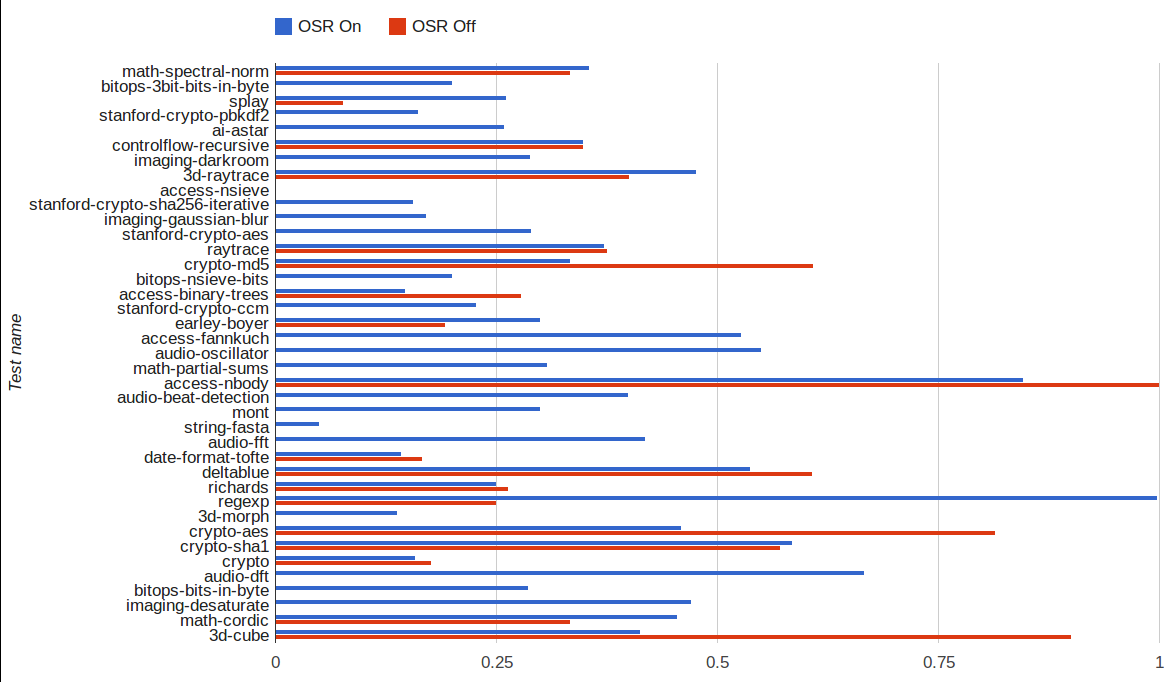
\includegraphics[width=0.98\textwidth]{counts_graph.png}
\caption{Fraction of add/subtract overflow checks eliminated}
\label{fig:count}
\end{figure*}


\section{Future Work and Conclusions}
We implement an SSA-based range analysis pass which is capable of
inferring range information on integer operations. We use the results
of this analysis to perform some simple optimizations relevant to
JavaScript: we eliminate overflow checks which can be proven
redundant, and also eliminate a limited number of array bounds checks.

On a suite of standard Javascript benchmarks, our range analysis
succeeds in eliminating a large fraction of overflow checks for
integer additions and subtractions. This translates into a minor
overall performance win on the Kraken benchmark suite and a very minor
overall performance loss on the SunSpider suite. Since we should only
increase the quality of the generated code, any performance losses
should be from increased compilation overhead (SunSpider tests in
particular are quite short). The performance improvements are decent,
but not stellar; we believe this is because Javascript code is
generally not integer-arithmetic-heavy tight loops and because the
overflow test branches are generally predicted correctly.

A number of further optimizations are possible using our range analysis
framework. If the range associated with an instruction becomes empty, then the
block has been proven dead and can be eliminated. Control flow operations can
be proven redundant as well, further eliminating computation and dead basic
blocks. These graph manipulations are currently not available in the IonMonkey
compiler, which is in active development but not yet complete. There are a
variety of reasons for this current design restriction. IonMonkey must
integrate very closely with the interpreter and the JS runtime, and so
generated code must maintain a careful correspondence with the interpreter.
This means that eliminating control flow is a non-trivial
operation\cite{dvander}.

Symbolic range propagation, where the bounds are expressed in terms of
definitions rather than integer constants, is left as future
work. Symbolic range propagation would allow more sophisticated
removal of bounds checks, which are generally not based on
constants. It would also allow for much more potential for eliminating
redundant branches than just constant ranges would.

We believe that we have implemented a worthwhile optimization and a
useful analysis pass that will serve as a good building block for
future IonMonkey optimizations. Our range analysis patches are likely
to land in IonMonkey in the next month, and it is likely that some of
the future work we discuss will be taken up by the IonMonkey team.

\bibliography{citations}{}
\bibliographystyle{abbrv}


\end{document}
